\documentclass[lettersize,journal]{IEEEtran}
\usepackage{amsmath,amsfonts}
\usepackage{amsthm}
\usepackage{algorithmic}
\usepackage{algorithm}
\usepackage{array}
\usepackage[caption=false,font=normalsize,labelfont=sf,textfont=sf]{subfig}
\usepackage{textcomp}
\usepackage{stfloats}
\usepackage{url}
\usepackage{verbatim}
\usepackage{graphicx}
\usepackage{cite}
\usepackage{multirow}
\hyphenation{op-tical net-works semi-conduc-tor IEEE-Xplore}
% updated with editorial comments 8/9/2021

\begin{document}

\title{Estimating Population Range by Recurring Online Chunk Bootstrap with Non-cumulative
Data in Streaming Data Environment}

\author{
\thanks{}}

%\author{Chidchanok Lursinsap${}^{1}$, Prem Jansawang${}^{2}$, Suphakant Phimoltares${}^{1}$ ~\IEEEmembership{}
        % <-this % stops a space
%\thanks{${}^{1}$Department of Mathematics and Computer Science, Faculty of Science, Chulalongkorn University, 
%Bangkok 10330, Thailand}% <-this % stops a space
%\thanks{${}^{2}$Department of Statistics, Faculty of Science, Khon Kaen University, Khon Kaen
%40002, Thailand}}

% The paper headers
%\markboth{Journal of \LaTeX\ Class Files,~Vol.~14, No.~8, August~2021}%
%{Shell \MakeLowercase{\textit{et al.}}: A Sample Article Using IEEEtran.cls for IEEE Journals}

\IEEEpubid{0000--0000/00\$00.00~\copyright~2021 IEEE}
% Remember, if you use this you must call \IEEEpubidadjcol in the second
% column for its text to clear the IEEEpubid mark.

\maketitle

\begin{abstract}

\end{abstract}

\begin{IEEEkeywords}
Article submission, IEEE, IEEEtran, journal, \LaTeX, paper, template, typesetting.
\end{IEEEkeywords}

\section{Introduction}
\IEEEPARstart{}{} 

\IEEEpubidadjcol



\section{Related Works and Concepts of Predicting Number of clusters}

This section summarized some interesting works relating to predicting the number of clusters based on 
distance analysis among data points.

\IEEEpubidadjcol



%\begin{figure*}[t]
%\centering
%\includegraphics[scale=0.6]{overview.eps}
%\vspace{-0.6in}
%\caption{Overview of proposed concept to identify actual number of clusters based on
%the observation of uniqueness of data distribution pattern and the finding of how the brain uses
%the past knowledge and experience to solve new problem.}  
%\label{overview}
%\end{figure*}

\section{Studied Problem and Objectives}

Let a chunk of integer data, a set of bins, and a set of integer data be defined as follows: 
\begin{enumerate}
\item A set of integer data, ${\bf D} = \{a \leq d_{j} \leq b \:\: | \:\: 1 \leq j \leq p\}$,
for integer constants $p$, $a$, and $b$.
\item An integer data chunk ${\bf C}$ divided into $n$ smaller chunks, 
${\bf C} = \{{\bf c}_{1}, \ldots, {\bf c}_{i}, \ldots, {\bf c}_{n} \:\: | \:\: 1 \leq n < \infty\}$. 
Each chunk has integers randomly taken from ${\bf D}$.
\item A bin ${\bf B}$ for containing incoming all integers in each chunk. There are two attributes, 
$v^{(min)}_{i}$ and $v^{(max)}_{i}$, defining the interval of integer values such that any integer 
$v^{(min)}_{i} \leq d_{j} \leq v^{(max)}_{i}$ can be assigned to this bin. 
\end{enumerate}
Each chunk ${\bf c}_{i}$ sequentially flows into the bin. If some integers whose values are
less than $v^{(min)}_{1}$ or larger than $v^{(max)}_{m}$, then the width of ${\bf B}$ must be expanded.

In the beginning, the size of bin ${\bf B}$ is made large enough to contain all integers in the first 
incoming chunk ${\bf c}_{1}$. Then size of ${\bf B}$ is occasionally expanded so that all integers in 
the other next incoming chunks can be assigned to the intervals of ${\bf B}$. Bin ${\bf B}$ is expanded 
if the values of some integers in some incoming chunks are either less than $v^{(min)}$ or larger 
than $v^{(max)}$. Therefore, the studied problem is defined as follows. 

Let $min({\bf D})$ and $max({\bf D})$ be the minimum and maximum values of ${\bf D}$. After capturing 
of integers in the first chunk, how to achieve the minimum number of expansions of ${\bf B}$ so that 
\begin{enumerate}
\item All incoming integers in the next other chunks can be assigned to ${\bf B}$.
\item $(min({\bf D}) - v^{(min)}_{1}) \geq 0$ is minimum.
\item $(v^{(max)}_{i} - max({\bf D})) \geq 0$ is minimum.
\end{enumerate}

\begin{figure}[!t]
\centering
%\resizebox{2.8in}{3.7in}{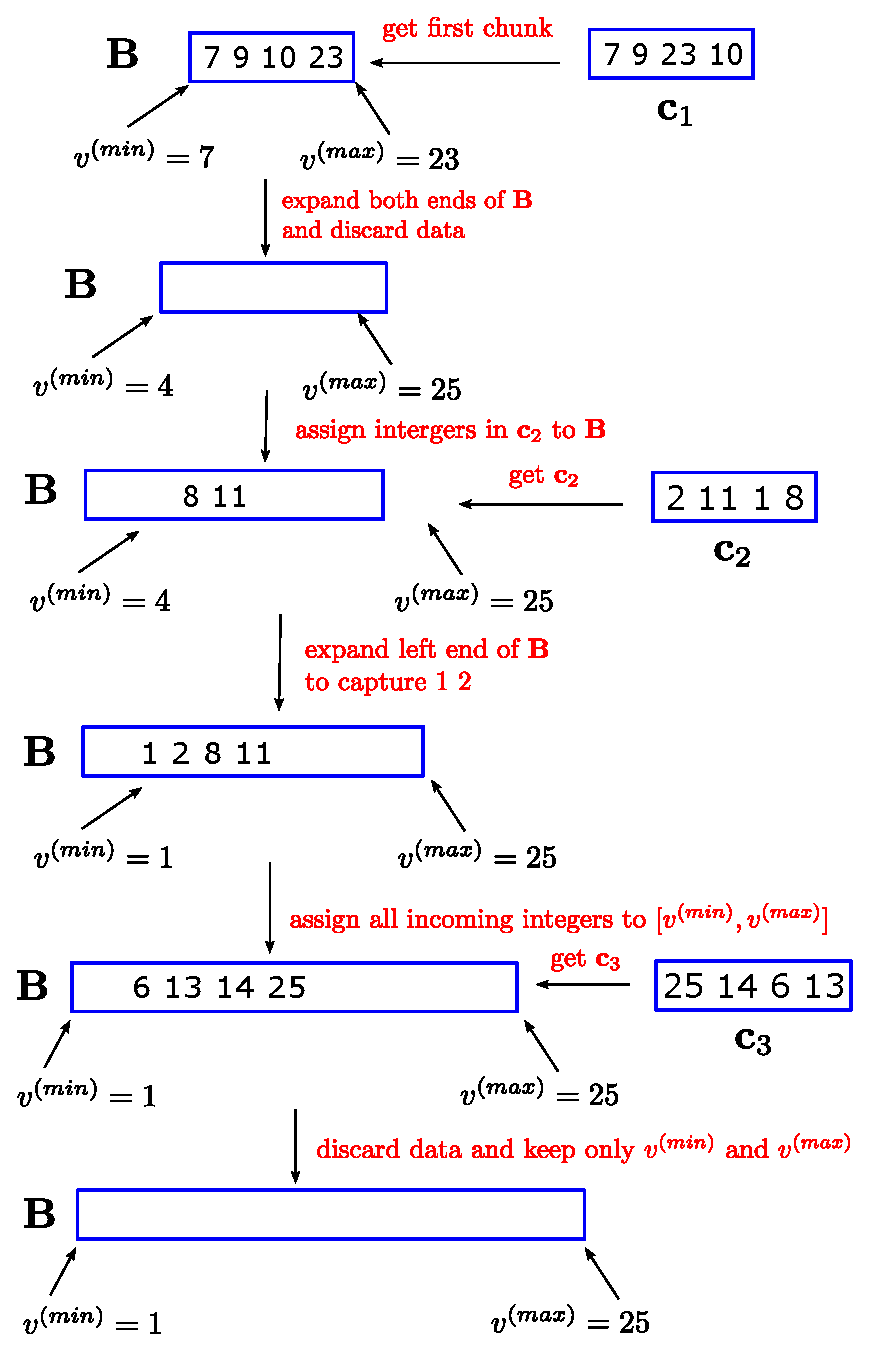
\includegraphics{example.eps}} 
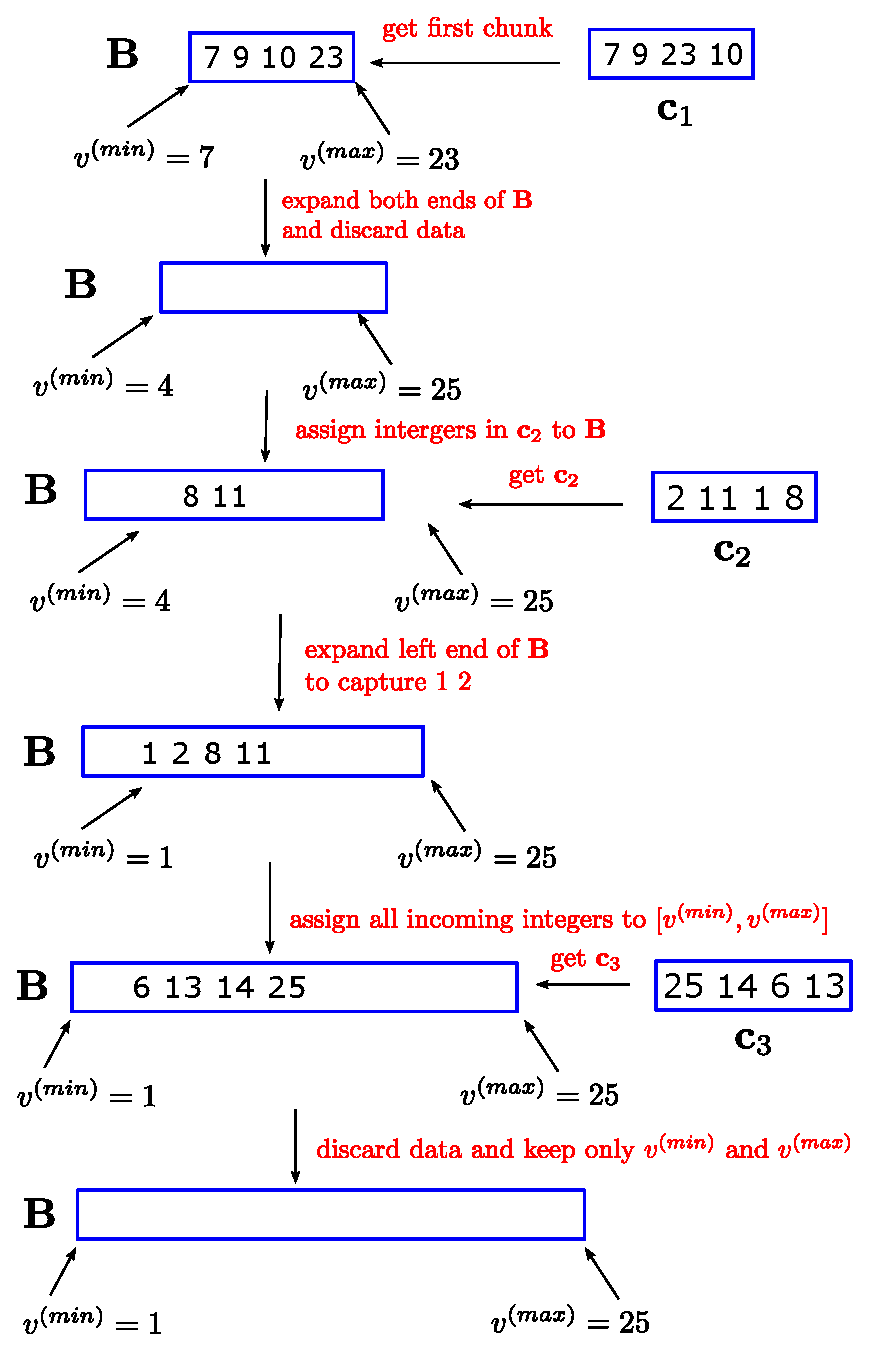
\includegraphics[scale = 0.5]{example.eps} 
\caption{An example of studied problem.} 
\label{example}
\end{figure}

\IEEEpubidadjcol
Figure \ref{example} illustrates an example scenario of capturing chunks. There are 3 sequentially incoming
chunks containing these integers: ${\bf c}_{1} = \{7, 9, 23, 10\}$, ${\bf c}_{2} = \{2, 11, 1, 8\}$,
${\bf c}_{3} = \{25, 14, 6, 13\}$. After capturing ${\bf c}_{1}$, the values of left and right ends of
bin ${\bf B}$ are set to $v^{(min)} = 7$ and $v^{(max)} = 23$ and all data are discarded. Then, both ends 
are expanded in advance to $v^{(min)}= 4$ and $v^{(max)} = 25$, preparing for ${\bf c}_{2}$. 
When ${\bf c}_{2}$ enters, all integers except 2 can be captured because the left end value 
$v^{(min)}= 4$ is larger than 2. Thus, the left end $v^{(min)}$ is expanded to $v^{(min)} = 2$. 
No need to expand the right end. All data in ${\bf c}_{2}$ are discarded. Then, get ${\bf c}_{3}$.
The interval of ${\bf B}$ is large enough to capture all integers of ${\bf c}_{3}$. After capturing 
${\bf c}_{3}$, all integers are discarded. In this example, the number of expansions is 2, after chunks 1 
and 2. Generally, how to achieve the minimum number of expansions of ${\bf B}$ in advance so that both
expanded values are also minimum.

\subsection{Constraints}
The amount of integers in each ${\bf c}_{i}$ is denoted by $|{\bf c}_{i}|$. Bin $B$ can be considered 
as an interval having left end denoted by $L$ and right end denoted by $R$. The following constraints are imposed.
\begin{enumerate}
\item The probability of distribution of each integer $d_{j}$ in ${\bf c}_{i}$ is unknown.
\item $|{\bf c}_{i}| \neq |{\bf c}_{i+1}|$ or $|{\bf c}_{i}| = |{\bf c}_{i+1}|$.
\item After assigning all integers of ${\bf c}_{i}$ inside the bin, chunk ${\bf c}_{i}$ is completely 
discarded and never reentered the bin assignment.
\end{enumerate}

\section{Concept of Recurring Online Bootstrap in Streaming Environment with Unrecorded Data}

\begin{figure*}[!th]
\centering
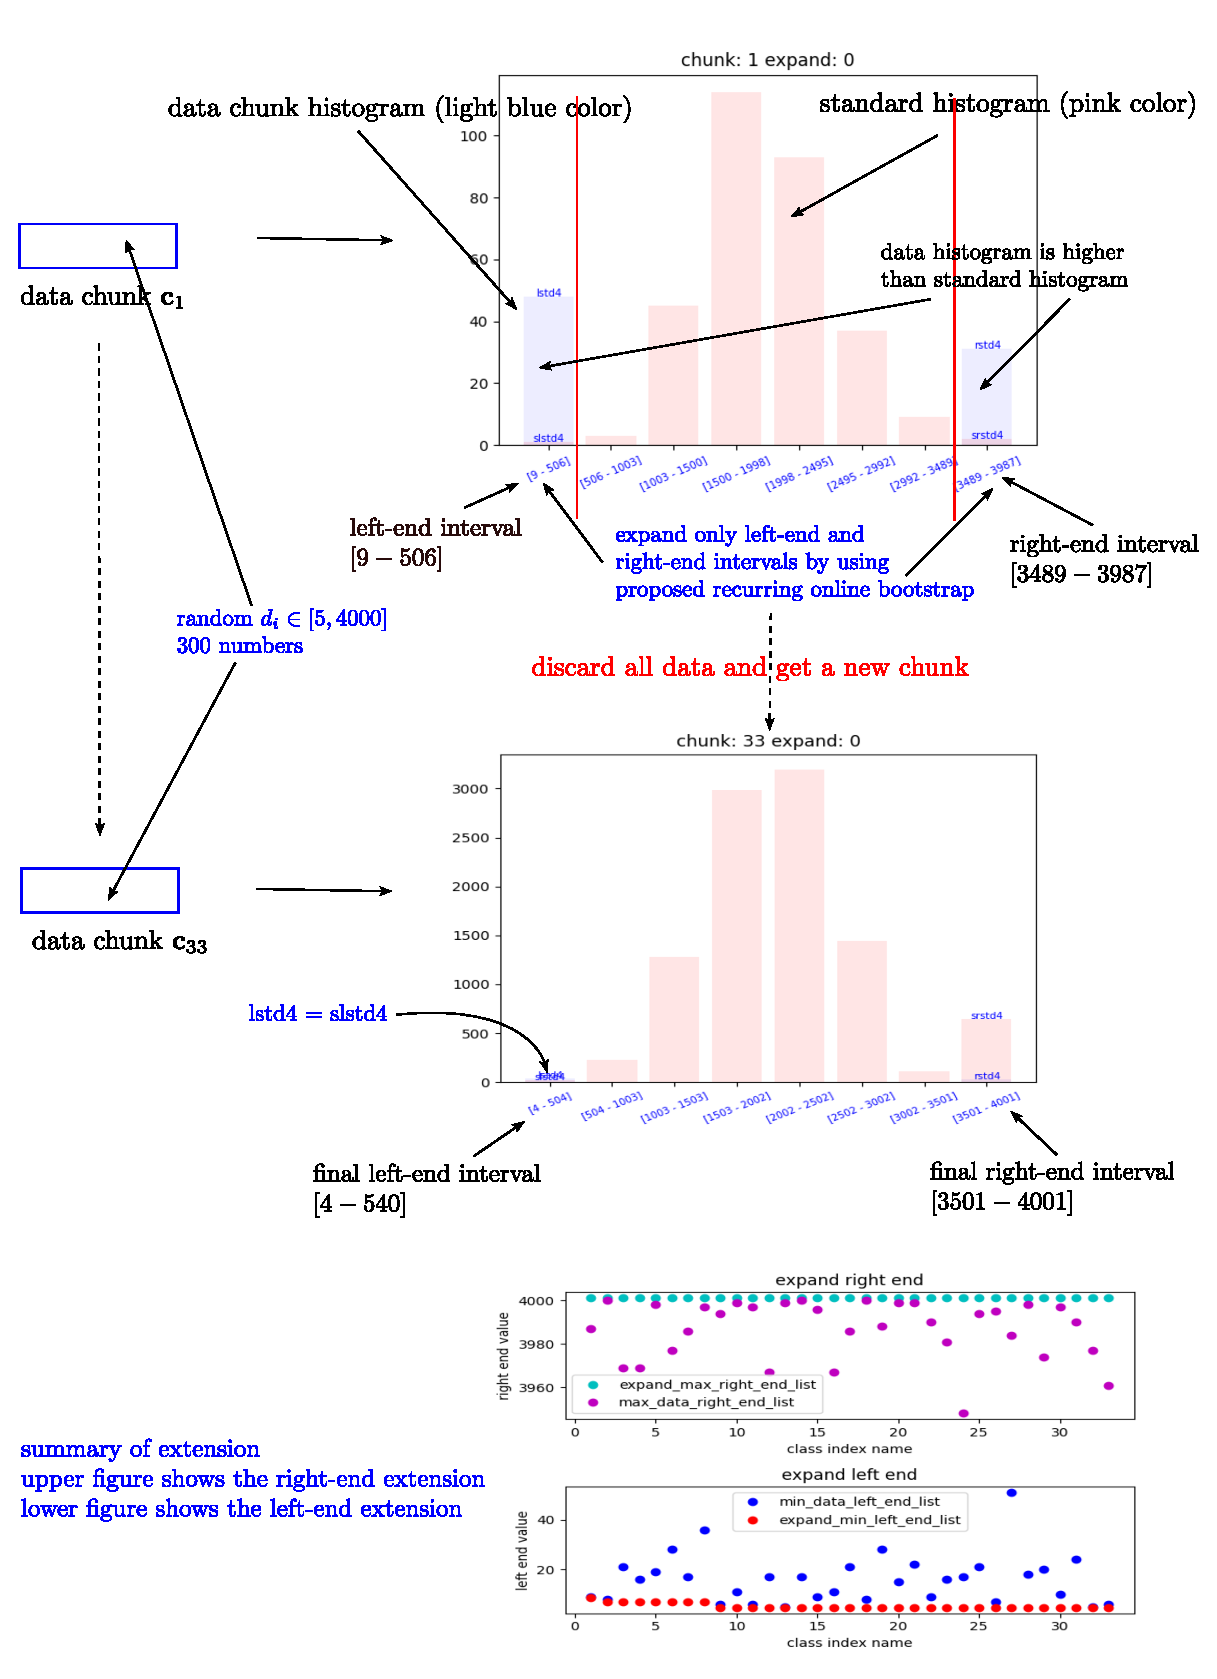
\includegraphics[scale = 0.7]{concept-framework.eps} 
\caption{Framework.} 
\label{frame-work}
\end{figure*}

\subsection{Algorithm}
explain standard histogram first 

The algorithm has two phases. The first phase

\vspace{0.2in}
\noindent
{\bf Algorithm 1:} Capturing data chunks and expanding ${\bf B}$ when it is necessary. \\

\noindent
{\bf Input:} Stream of data chunks, ${\bf c}_{i}$ for $1 \leq i < \infty$. \\
{\bf Output:}

\vspace{0.2in}
\noindent
{\bf Phase 1:} Capturing ${\bf c}_{1}$ and get initial expansion of ${\bf B}$.

\begin{tabbing}
1.~~ \= Get ${\bf c}_{1}$ and set $total\_data = |{\bf c}_{1}|$. \\
2.~~ \> Let $v^{(min)} = \min({\bf c}_{1})$ and $v^{(max)} = \max({\bf c}_{1})$. \\
3.~~ \> Divide ${\bf B}$ into 8 equal sub-intervals ${\bf b}_{i}$ for $1 \leq i \leq 8$, \\
     \> each of size $(v^{(max)} - v^{(min)})/8$. \\
4.~~ \> Put the integers in ${\bf c}_{1}$ whose values are within \\
     \> sub-intervals ${\bf b}_{1}$ and ${\bf b}_{8}$ into these two sub-intervals. \\
5.~~ \> Count the number of integers in ${\bf b}_{1}$ and ${\bf b}_{8}$  \\
     \> and let $|{\bf b}_{1}|$ and $|{\bf b}_{8}|$ denote these numbers. \\
6.~~ \> Let $avg = (v^{(max)} + v^{(min)})/2$ be the middle value of \\
     \> ${\bf B}$. \\
7.~~ \> Find the types of probability distribution in list $P$ \\
     \> best fitting the data in ${\bf b}_{1}$, and ${\bf b}_{8}$ by using Algorithm \\
     \> 2.1 with $total\_data$, ${\bf b}_{1}$, and ${\bf b}_{8}$. \\
8.~~ \> Compute the standard number of integers in ${\bf b}_{1}$ \\
     \> denoted by $lstd$, and in ${\bf b}_{8}$ denoted by $rstd$. \\
     \> from the best fitted probability distribution by \\
     \> using Algorithm 2.2. \\
9.~~ \> ${\bf While}$ \= $|{\bf b}_{1}| > lstd$ or $|{\bf b}_{8}| > rstd$ ${\bf do}$ \\
10.~~ \>               \> ${\bf If}$ \= $|{\bf b}_{1}| > lstd$ ${\bf then}$ \\
11.~~\>               \>            \> Expand $v^{(min)}$ by using Algorithm 3 with \\
     \>               \>            \> all integers in ${\bf b}_{1}$. \\
12.~~\>               \> ${\bf EndIf}$ \\
13.~~\>               \> ${\bf If}$ \= $|{\bf b}_{8}| > rstd$ ${\bf then}$ \\
14.~~\>               \>            \> Expand $v^{(max)}$ by using Algorithm 4 with \\
     \>               \>            \> all integers in ${\bf b}_{8}$. \\
15.~~\>               \> ${\bf EndIf}$ \\
16.~~\>               \> Adjust the width of ${\bf b}_{1}$ and ${\bf b}_{8}$ by dividing ${\bf B}$ \\
     \>               \> into 8 equal sub-intervals ${\bf b}_{i}$ for $1 \leq i \leq 8$, \\
     \>               \> each of size $(v^{(max)} - v^{(min)})/8$. \\
17.~~\> ${\bf EndWhile}$ \\
18.~~\> Discard ${\bf c}_{1}$ and all integers in ${\bf b}_{1}$ and ${\bf b}_{8}$.
\end{tabbing}

\vspace{0.2in}
\noindent
{\bf Phase 2:} Capturing other ${\bf c}_{i}$ and determining the necessity of expanding ${\bf B}$.
\begin{tabbing}
1.~~ \= ${\bf while}$ \= there exists a new incoming chunk ${\bf c}_{i}$ ${\bf do}$ \\
2.~~ \>               \> $total\_data = total\_data + |{\bf c}_{i}|$. \\
3.~~ \>               \> ${\bf If}$ \= $\min({\bf c}_{i}) < v^{(min)}$ ${\bf then}$ \\
4.~~ \>               \>          \> $v^{(min)} = \min({\bf c}_{i})$. \\
5.~~ \>               \> ${\bf EndIf}$. \\
6.~~ \>               \> ${\bf If}$ \= $v^{(max)} < \max({\bf c}_{i})$ ${\bf then}$ \\
7.~~ \>               \>          \> $v^{(max)} = \max({\bf c}_{i})$. \\
8.~~ \>               \> ${\bf EndIf}$. \\
9.~~ \>               \> Divide ${\bf B}$ into 8 equal sub-intervals ${\bf b}_{i}$ for \\
     \>               \> $1 \leq i \leq 8$, each of size $(v^{(max)} - v^{(min)})/8$. \\
10.~~\>               \> Put the integers in ${\bf c}_{i}$ whose values are within \\
     \>               \> sub-intervals ${\bf b}_{1}$ and ${\bf b}_{8}$ into these two \\
     \>               \> sub-intervals. \\
11.~~\>               \> Count the number of integers in ${\bf b}_{1}$ and ${\bf b}_{8}$  \\
     \>               \> and let $|{\bf b}_{1}|$ and $|{\bf b}_{8}|$ denote these numbers. \\
12.~~\>               \> Find the types of probability distribution in list $P$ \\
     \>               \> best fitting the data in ${\bf b}_{1}$, and ${\bf b}_{8}$ by using \\
     \>               \> Algorithm 2.1 with $total\_data$, ${\bf b}_{1}$, and ${\bf b}_{8}$. \\
13.~~\>               \> Compute the standard number of integers in ${\bf b}_{1}$ \\
     \>               \> denoted by $lstd$, and in ${\bf b}_{8}$ denoted by $rstd$ \\
     \>               \> from the best fitted probability distribution by \\
     \>               \> using Algorithm 2.2. \\
14.~~\>               \> ${\bf While}$ \= $|{\bf b}_{1}| > lstd$ or $|{\bf b}_{8}| > rstd$ ${\bf do}$ \\
15.~~\>               \>               \> ${\bf If}$ \= $|{\bf b}_{1}| > lstd$ ${\bf then}$ \\
16.~~\>               \>               \>            \> Expand $v^{(min)}$ by using Algorithm 3 \\
     \>               \>               \>            \> with all integers in ${\bf b}_{1}$. \\
17.~~\>               \>               \> ${\bf EndIf}$ \\
18.~~\>               \>               \> ${\bf If}$ \= $|{\bf b}_{8}| > rstd$ ${\bf then}$ \\
19.~~\>               \>               \>            \> Expand $v^{(max)}$ by using Algorithm 4 \\
     \>               \>               \>            \> with all integers in ${\bf b}_{8}$. \\
20.~~\>               \>               \> ${\bf EndIf}$ \\
21.~~\>               \>               \> Adjust the width of ${\bf b}_{1}$ and ${\bf b}_{8}$ by dividing\\
     \>               \>               \> ${\bf B}$ into 8 equal sub-intervals ${\bf b}_{i}$ for \\
     \>               \>               \> $1 \leq i \leq 8$, each of size {\small 
                                          $(v^{(max)} - v^{(min)})/8$}. \\
22.~~\>               \> ${\bf EndWhile}$. \\
23.~~\>               \> Discard ${\bf c}_{i}$ and all integers in ${\bf b}_{1}$ and ${\bf b}_{8}$. \\
24.~~\> ${\bf EndWhile}$.      
\end{tabbing}

\vspace{0.2in}
\noindent
{\bf Algorithm 2.1:} Finding the types of probability distribution in list $P$ best fitting the data in 
${\bf b}_{1}$, and ${\bf b}_{8}$.

\noindent
{\bf Input:} (1) A list of standard probability distribution $P$. (2) $total\_data$. (3) ${\bf b}_{1}$.
(4) ${\bf b}_{8}$. \\
{\bf Output:} $lname$ and $rname$.

\vspace{0.2in}
\noindent

\begin{tabbing}

1.~~ \= ${\bf For}$ \= each type probability distribution $p \in P$ ${\bf do}$ \\
2.~~ \>             \> Divide the area under standard probability \\
     \>             \> distribution $p$ into 8 stripes of equal width. \\
3.~~ \>             \> Let $l^{(p)}_{4}$ be the percentage of data in the $4^{th}$ stripe \\
     \>             \> to the left of mean. \\
4.~~ \>             \> Let $r^{(p)}_{4}$ be the percentage of data in the $4^{th}$ stripe \\
     \>             \> to the right of mean.\\
5.~~ \>             \> Compute the difference between standard number \\
     \>             \> of integers in the $4^{th}$ left stripe and $|{\bf b}_{1}|$: \\
     \>             \> $ld^{(p)} = abs(l^{(p)}_{4} * total\_data - |{\bf b}_{1}|)$. \\
6.~~ \>             \> Compute the difference between standard number \\
     \>             \> of integers in the $4^{th}$ right stripe and $|{\bf b}_{8}|$: \\
     \>             \> $rd^{(p)} = abs(r^{(p)}_{4} * total\_data - |{\bf b}_{8}|)$. \\
7.~~ \> ${\bf EndFor}$ \\
8.~~ \> Find $lname = \arg \min\limits_{p \in P} (ld^{(p)})$. \\
9.~~ \> Find $rname = \arg \max\limits_{p \in P} (rd^{(p)})$. \\
10.~~\> ${\bf Return}$ $lname$ and $rname$.
\end{tabbing}

\vspace{0.2in}
\noindent
{\bf Algorithm 2.2:} Computing $lstd$ and $rstd$. \\

\noindent
{\bf Input:} (1) A list of standard probability distribution $P$. (2) $total\_data$. (3) $lname$.
(4) $rname$. (5) $l^{(p)}_{4}$ and $r^{(p)}_{4}$; $\forall p \in P$ from Algorithm 2.1. \\
{\bf Output:} $lstd$ and $rstd$.

\begin{tabbing}
1.~~\= ${\bf If}$ \= $lname$ is the same as $rname$ ${\bf then}$ \\
2.~~\>            \> Set $lstd = l^{(lname)}_{4} * total\_data$. \\
3.~~\>            \> Set $rstd = r^{(rname)}_{4} * total\_data$. \\
4.~~\> ${\bf EndIf}$ \\
5.~~\> ${\bf If}$ \= $lname$ is different from $rname$ ${\bf then}$ \\
6.~~\>            \> Set $lstd = \max\limits_{p \in P} (l^{(p)}_{4}) * total\_data$. \\ 
7.~~\>            \> Set $rstd = \max\limits_{p \in P} (r^{(p)}_{4}) * total\_data$. \\ 
8.~~\> ${\bf EndIf}$ \\
9.~~\> ${\bf Return}$ $lstd$ and $rstd$.
\end{tabbing}

\vspace{0.2in}
\noindent
{\bf Algorithm 3:} Recurring online chunk bootstrap for ${\bf B}_{1}$. \\

\noindent
{\bf Input:} (1) Present set of incoming integers in ${\bf B}_{1}$; (2) Number of bootstrap iterations 
$N$; (3) $mean({\bf a})$ is a function computing the mean of set ${\bf a}$; (4) $std({\bf a})$ is a 
function computing the standard deviation of set ${\bf a}$; (5) $abs(x)$ is the absolute value of 
constant $x$. \\
{\bf Output:} $v^{(min)}$.

\begin{tabbing}
1.~~ \= Let ${\bf S} = \emptyset$ be a set of bootstrapped samples. \\
2.~~ \> Let ${\bf M} = \emptyset$ be a set of mean of each bootstrapped \\
     \> sample. \\
3.~~ \> Let ${\bf P} = \emptyset$ be a set of standard deviation of each \\
     \> bootstrapped sample. \\
4.~~ \> $prev\_mean = 0$. \\
5.~~ \> ${\bf For}$ \= $1 \leq i \leq N$ ${\bf do}$: \\
6.~~ \>             \> Let ${\bf s}_{i}$ be a set of randomly sampled integers of \\
     \>             \> size $|{\bf B}_{1}|$ from ${\bf B}_{1}$ with replacement. \\
7.~~ \>             \> ${\bf S} = {\bf S} \cup \{{\bf s}_{i}\}$. \\
8.~~ \>             \> $present\_mean = (mean({\bf s}_{i}) + prev\_mean)/2$. \\
9.~~ \>             \> $prev\_mean = present\_mean$. \\
10.~~\>             \> ${\bf M} = {\bf M} \cup \{present\_mean\}$. \\
11.~~\> ${\bf EndFor}$. \\
12.~~\> $\mu^{(boot)} = mean({\bf M})$. \\
13.~~\> ${\bf For}$ \= each ${\bf s}_{i} \in {\bf S}$ ${\bf do}$ \\
14.~~\>             \> ${\bf P} = {\bf P} \cup \{std({\bf s}_{i})\}$. \\
15.~~\> ${\bf EndFor}$ \\
16.~~\> $\sigma^{(boot)} = mean({\bf P})$. \\
17.~~\> $\mu^{(diff)} = abs(mean({\bf B}_{1}) - \mu^{(boot)})$. \\
18.~~\> $\sigma^{(diff)} = abs(std({\bf B}_{1}) - \sigma^{(boot)})$. \\
19.~~\> ${\bf If}$ \= $mu^{(boot)} < mean({\bf B}_{1}$) ${\bf do}$ \\
20.~~\>            \> $v^{(min)} = min({\bf B}_{1}) - \mu^{(diff)}$. \\ 
21.~~\> ${\bf If}$ \= $mean({\bf B}_{1}) < mu^{(boot)}$ ${\bf do}$ \\
22.~~\>            \> $v^{(min)} = min({\bf B}_{1}) - \sigma^{(diff)}$. \\ 
\end{tabbing}


\vspace{0.2in}
\noindent
{\bf Algorithm 4:} Recurring online chunk bootstrap for ${\bf B}_{8}$. \\

\noindent
{\bf Input:} (1) Present set of incoming integers in ${\bf B}_{1}$; (2) Number of bootstrap iterations 
$N$; (3) $mean({\bf a})$ is a function computing the mean of set ${\bf a}$; (4) $std({\bf a})$ is a 
function computing the standard deviation of set ${\bf a}$; (5) $abs(x)$ is the absolute value of 
constant $x$. \\
{\bf Output:} $v^{(max)}$.

\begin{tabbing}
1.~~ \= Let ${\bf S} = \emptyset$ be a set of bootstrapped samples. \\
2.~~ \> Let ${\bf M} = \emptyset$ be a set of mean of each bootstrapped \\
     \> sample. \\
3.~~ \> Let ${\bf P} = \emptyset$ be a set of standard deviation of each \\
     \> bootstrapped sample. \\
4.~~ \> $prev\_mean = 0$. \\
5.~~ \> ${\bf For}$ \= $1 \leq i \leq N$ ${\bf do}$: \\
6.~~ \>             \> Let ${\bf s}_{i}$ be a set of randomly sampled integers of \\
     \>             \> size $|{\bf B}_{8}|$ from ${\bf B}_{8}$ with replacement. \\
7.~~ \>             \> ${\bf S} = {\bf S} \cup \{{\bf s}_{i}\}$. \\
8.~~ \>             \> $present\_mean = (mean({\bf s}_{i}) + prev\_mean)/2$. \\
9.~~ \>             \> $prev\_mean = present\_mean$. \\
10.~~\>             \> ${\bf M} = {\bf M} \cup \{present\_mean\}$. \\
11.~~\> ${\bf EndFor}$. \\
12.~~\> $\mu^{(boot)} = mean({\bf M})$. \\
13.~~\> ${\bf For}$ \= each ${\bf s}_{i} \in {\bf S}$ ${\bf do}$ \\
14.~~\>             \> ${\bf P} = {\bf P} \cup \{std({\bf s}_{i})\}$. \\
15.~~\> ${\bf EndFor}$ \\
16.~~\> $\sigma^{(boot)} = mean({\bf P})$. \\
17.~~\> $\mu^{(diff)} = abs(mean({\bf B}_{8}) - \mu^{(boot)})$. \\
18.~~\> $\sigma^{(diff)} = abs(std({\bf B}_{8}) - \sigma^{(boot)})$. \\
19.~~\> ${\bf If}$ \= $mu^{(boot)} < mean({\bf B}_{8}$) ${\bf do}$ \\
20.~~\>            \> $v^{(max)} = min({\bf B}_{8}) + \sigma^{(diff)}$. \\ 
21.~~\> ${\bf If}$ \= $mean({\bf B}_{1}) < mu^{(boot)}$ ${\bf do}$ \\
22.~~\>            \> $v^{(max)} = min({\bf B}_{8}) + \mu^{(diff)}$.
\end{tabbing}

\begin{thebibliography}{1}
\bibliographystyle{IEEEtran}

\bibitem{hong}
Hong Yu, Zhanguo Liu, Guoyin Wang, ``An automatic method to determine the number of clusters using
decision-theoretic rough set'', International Journal of Approximate Reasoning 55 (2014) 101–115.
%\bibitem{}



\end{thebibliography}


\newpage

%\section{Biography Section}
%If you have an EPS/PDF photo (graphicx package needed), extra braces are
% needed around the contents of the optional argument to biography to prevent
% the LaTeX parser from getting confused when it sees the complicated
% $\backslash${\tt{includegraphics}} command within an optional argument. (You can create
% your own custom macro containing the $\backslash${\tt{includegraphics}} command to make things
% simpler here.)
 
%\vspace{11pt}

%\bf{If you include a photo:}\vspace{-33pt}
%\begin{IEEEbiography}[{\includegraphics[width=1in,height=1.25in,clip,keepaspectratio]{fig1}}]{Michael Shell}
%Use $\backslash${\tt{begin\{IEEEbiography\}}} and then for the 1st argument use $\backslash${\tt{includegraphics}} to declare and link the author photo.
%Use the author name as the 3rd argument followed by the biography text.
%\end{IEEEbiography}

\vspace{11pt}

%\bf{If you will not include a photo:}\vspace{-33pt}
%\begin{IEEEbiographynophoto}{John Doe}
%Use $\backslash${\tt{begin\{IEEEbiographynophoto\}}} and the author name as the argument followed by the biography text.
%\end{IEEEbiographynophoto}




%\vfill

\end{document}


